129. \begin{figure}[ht!]
\center{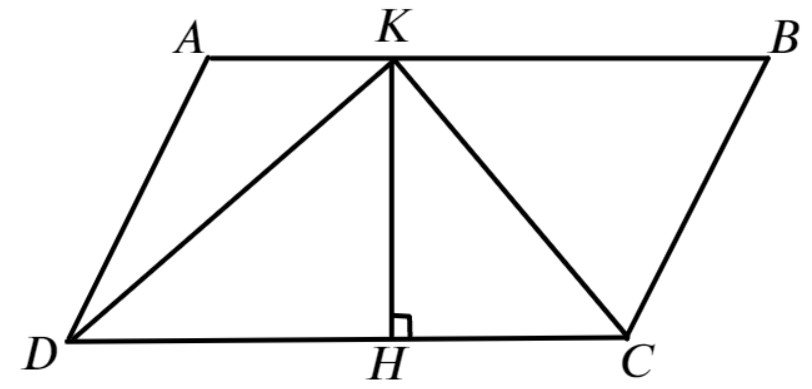
\includegraphics[scale=0.35]{g8-129.png}}
\end{figure}\\
Опусти высоту $KH$ из точки $K,$ она равна также и высоте параллелограмма. Тогда $S_{\Delta CDK}=\cfrac{1}{2}\cdot KH\cdot CD,\ S_{ABCD}=KH\cdot CD\Rightarrow
S_{ABCD}=2S_{\Delta CDK}=56.$\\
